\documentclass[11pt]{article}  
\usepackage[margin=1in]{geometry}
\usepackage{authblk}
\usepackage{graphicx}
\usepackage{amsmath}

\usepackage{ltexpprt} 

\begin{document}
\title{Multi-Commodity Flow with In-Network Processing}
%\thanks{Supported by .} 
\author[]{Moses Charikar}
\author[]{Yonatan Naamad}
\author[]{Jennifer Rexford}
\author[]{X. Kelvin Zou}
\affil[]{Department of Computer Science, Princeton University}
\affil[ ]{\textit {\{moses,ynaamad,jrex, xuanz\}@cs.princeton.edu}}
\date{}
\maketitle

\section{Introduction}
\subsection{Background}
Networks have evolved beyond a simple packet forwarding. Many types of in-network flow processing are ubiquitous today. The flow processing usually take place at vertices, in which we install one or a few appliances, so called middleboxes(MBoxes), examples including firewall, encryption and compression. In many cases the flow has to go through a sequence of MBox processing in order to fulfill the function or security requirements. 

Traditionally, these MBoxes use specialized hardware and are installed at predetermined locations(vertices). In terms of the locations, some design places MBoxes at juncture points(e.g., gateways) in special network topologies such as FatTree\cite{FATTREE}, but it leads to inefficient routing in cases where the both source and sink are sharing the same predecessors. It also fails to cover generalized networks or enforce the policy for a sequence of MBoxes.

The recent development of MBox virtualization enables more flexible deployment. MBoxes are no longer hardware dependent and can be spin up(or down) at any physical server\cite{clickos, ANANTA2013}. In this new architecture, the processing capacities are homogeneous and the problem becomes simply where to place MBox servers. There are two choices: 1. separate the server placement and routing decision: place MBox servers first and make routing decisions based on MBox locations\cite{SIMPLE2013}; 2. have a joint optimization scheme where the server locations are decided based on potential routing decisions given the flow demand. We argue that the latter is better in terms of efficiency but imposes the hardness for the server placement. 
\subsection{The Problem}
We can abstract the flow in-network process problem in the following way: there is a flow demand with multi-sources and multi-sinks, and each flow requires a certain amount of in-network (MBox) processing. The in-network processing required for a flow is proportional to the flow size and without losing generality, we assume one unit of flow requires one unit of processing. For a flow from a source to a sink, we assume it is an aggregate flow so the routing and in-network processing for a flow are both divisible. In this model there are two types of constraints: edge capacity and vertex capacity, which represents bandwidth and MBox processing capacity. A feasible flow pattern satisfies: the sum of flows on each edge is bounde by the edge capacity, the sum of in-network process done at each vertex is bounded by the vertex capacity, and the processing done at all vertices for a flow should be equal to flow size and the processing has to be carried out by the flow.

Network design problems involve finding a network with a minimum cost that satisfies various properties, often related to routing and flow feasibility. The network design problem in this model is: for a multi-source and multi-sink flow demand, and a fixed amount of budget to install the processing capacities in the vertices, what is the optimal way to allocate them such that the flow pattern satisfies all the constraints.

Our model is a superset of multi-commodity flow model\cite{MCF}, that is, if we can solve this problem, we can naturally solve multi-commodity flow problem: simply assign each vertex with an infinite capacity it becomes an MCF problem. Many classic MCF design properties can be extended to this problem, such as MC-BB(multi-commodity buy-at-bulk) problem\cite{BuyAtBulk,Charikar05,Chekuri2007}. 
%This paper takes the second approach and show that the decision can be answered via generalized linear programming model for a fractional solution, and have a logarithm approximation for a more practical integer placement.

\begin{figure}[h]
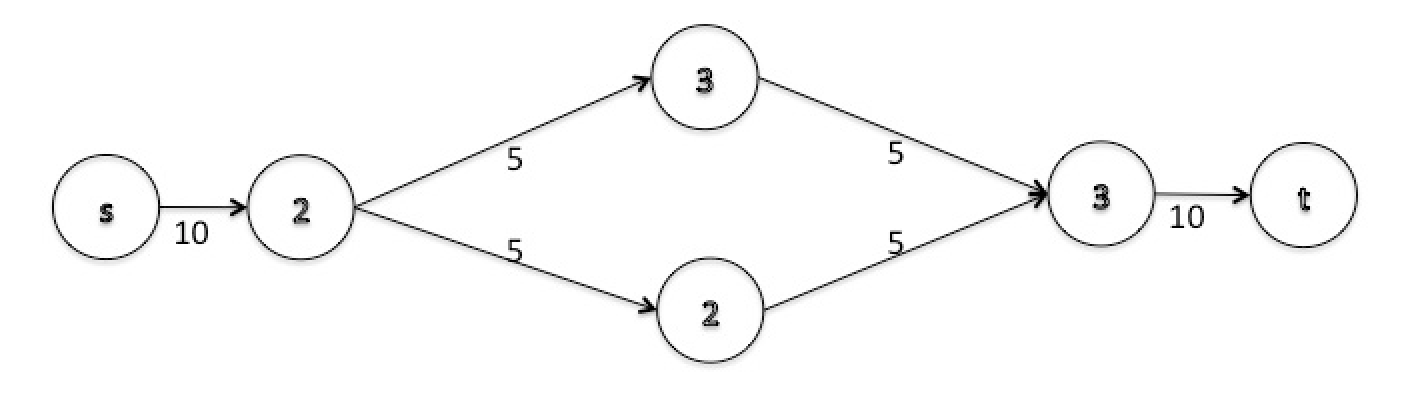
\includegraphics[width=\linewidth]{picture1.png} 
\caption{ \textbf{Example for the Graph Model: given the edge and vertex constraints, \textnormal{\{5,10\} }are edge capacities and \{2,3\} are vertex capacities, the maximum flow from source to sink in the example is 10, in this example all edges and vertices will be saturated.} }
 \end{figure}
\subsection{Notations}
To capture both the capacitated vertices and edges, we use the following notations:
a directed graph $G(V,E)$ where each edge $e\in E$ has an edge bandwidth $B(e)$, and each vertex $v\in V$ has a processing capacity $C(v)$. 

 


\subsection{The results in this paper}



\section{Processing Capacity Placement in fractional manner}
We formulate a generalized linear programming model in this problem in an edge based formulation. Notations: $C(v),B(e)$ represents the processing and edge capacity at node $v$ and edge $e$, $f_i(e)$ represents the flow size for each source-sink pair on edge $e$, $w_i(e)$ represents process demand for flow i carried out at edge $e$, $f(C(v))$ is an concave cost function of $C(v)$: 

\begin{subequations}
\begin{align}
\text{Minimize:}&\sum\limits_v f(C(v))\\
\text{Subject to:}&\forall v \in V-\{s, t\}, \forall i, \sum\limits_{in}  f_i(e)=  \sum\limits_{out} f_i(e);\\
&\forall e, \sum\limits_{i} f_{i}(e)\leq B(e);\\
&\forall e,\forall  i,0 \leq w_i(e) \leq f_i(e),\\
&\forall v,\forall  i, 0\leq \sum\limits_{in } w_i(e) - \sum\limits_{out} w_i(e)   \leq{C(v)}.\\
%&\forall i, \sum\limits_v f_i(s, v) = r_i; \\
&\forall  i; \forall (s, v), w_i = f_i\;\&\; \forall (v,t), w_i =0.
\end{align}
\end{subequations}




\bibliographystyle{acm}
\bibliography{references}

\appendix
\end{document}